% 4章
\chapter{モデルの検証}

本章では,高齢者施設を模した介護空間が環境として設定できているか,使用した歩行者モデルのSocial Force Modelが正しく動いているか,作成したシミュレータの中で介護シミュレーションが正しく機能しているかについて検証する.Social Force Modelの検証では,歩行者しかいない環境における基本的な可視化をおこない,目的への斥力や他エージェントからの斥力が働いているかを確認する.介護シミュレーションの検証では,被介護者がアラートを出した時に介護者が経路選択を行い,あらかじめ設定した介護行動が行われるかを可視化する.また、複数の介護アラートが発生した時に,あらかじめ設定したロジックに基づき介護対象を選択できるかについても検証を行う.

\section{環境設定の検証}

環境設定の検証は,いくつかの二次元平面を実際に作成し,可視化することで行う.また,その中で介護者・被介護者も同様に可視化する.被介護者は通常状態とアラートを出している状態で色を変える.まずは図\ref{environment_v1}にあるように,簡単な二次元平面と歩行者を可視化した.次に,図\ref{environment_v2}のように,同じ二次元空間の中で,介護者と被介護者を可視化し,被介護者の状態によって色が変わった状態も可視化できた.同様に車椅子に乗っている被介護者を想定した被介護者エージェントや,技術によるサポートを受けている被介護者を想定した被介護者エージェントも同様に,色や形を変えることで表現することができる.本シミュレータでは,介護空間を記述するための必要条件である,二次元平面と介護者,被介護者を再現することができると言える.

\begin{figure}[htb]
\begin{center}
 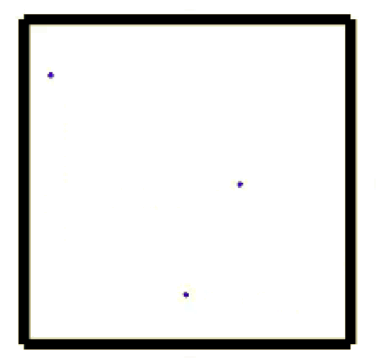
\includegraphics[scale=0.4]{figures/environment_v1}
 \caption[二次元空間の可視化]{二次元空間の可視化 \label{environment_v1}}
\end{center}
\end{figure}

\begin{figure}[htb]
\begin{center}
 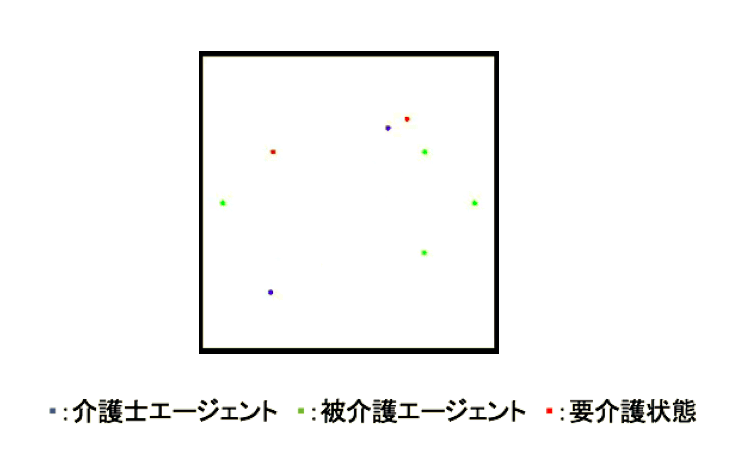
\includegraphics[scale=0.4]{figures/environment_v2}
 \caption[介護者・被介護者の可視化]{介護者・被介護者の可視化 \label{environment_v2}}
\end{center}
\end{figure}

\section{Social Force Modelの検証}

Social Force Modelの検証は,環境設定の検証で作成した環境とは異なる二次元空間を作成し,その中でエージェント同士の相互作用が行われているかを確認する.歩行者エージェント作成し,手入力で目的地の配列を初期条件として与え,一定時間ごとに同じスタート地点にエージェントを発生させ,同じ経路を設定する.現在地から目的地までは,Social Force Modelで定義されている目的地に向かう力と他のエージェントからの斥力,壁からの斥力,魅力的な場所からの引力(本検証では用いない)の合力が働くので,例えば同じ経路上ですれ違う場合は,たとえ経路が同じであったとしても互いが互いを避けて通るようになるはずである.

まずは,環境として図\ref{SFM_environment}を準備する.二次元空間の中に壁を作成し,1の位置から歩行者エージェントが一定時間ごとに発生するようにする.歩行者エージェントは,1から順番に1,2,3,4,3,2,5,2,1,6という経路の目的地群を与え,現在の目的地であるサブゴールに到着すると,次の目的に向かって移動していく.

\begin{figure}[htb]
\begin{center}
 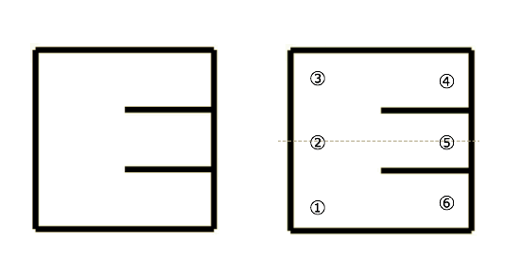
\includegraphics[scale=0.6]{figures/SFM_environment}
 \caption[SFMの検証における環境設定]{SFMの検証における環境設定 \label{SFM_environment}}
\end{center}
\end{figure}

その様子を図\ref{SFM_visual}に可視化した.シミュレーションでは,目的地に到着後,壁にぶつからないように折り返し,他のエージェントとすれ違う際に,目的地間の最短経路を通らず,お互いがお互いを避ける挙動を確認することができた.本シミュレータでは,介護空間を記述するための必要条件である,経路選択と目的地までの移動を再現することができると言える.

\begin{figure}[htb]
\begin{center}
 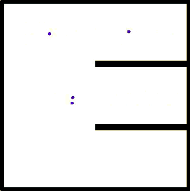
\includegraphics[scale=0.6]{figures/SFM_visual}
 \caption[SFMの検証における可視化結果]{SFMの検証における可視化結果 \label{SFM_visual}}
\end{center}
\end{figure}

\section{介護シミュレーションの検証}

本章では最後に,介護シミュレーションについての検証を行う.本シミュレーションでは,被介護者のバリエーションとして以下の3種類を実装している.

\begin{itemize}
 \item 適切なタイミングで介護アラートを出すエージェント
 \item 早いタイミングで介護アラートを出すエージェント
 \item 遅いタイミングで介護アラートを出すエージェント
\end{itemize}

本研究では、排泄介助を対象としているので、適切なタイミングで介護アラートを出すエージェントを健常者(技術のサポートを受けている被介護者),早いタイミングで介護アラートを出すエージェントを頻尿の被介護者,遅いタイミングで介護アラートを出すエージェントを認知症の被介護者と呼ぶことにする.それぞれを可視化した図が,図\ref{elderly_v1},図\ref{elderly_v2},図\ref{elderly_v3}である.

\begin{figure}[htb]
\begin{center}
 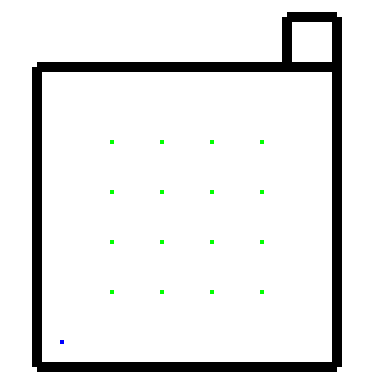
\includegraphics[scale=0.5]{figures/elderly_v1.png}
 \caption[健常者(介護技術を導入した場合の被介護者)の場合の可視化]{健常者(介護技術を導入した場合の被介護者)の場合の可視化 \label{elderly_v1}}
\end{center}
\end{figure}

\begin{figure}[htb]
\begin{center}
 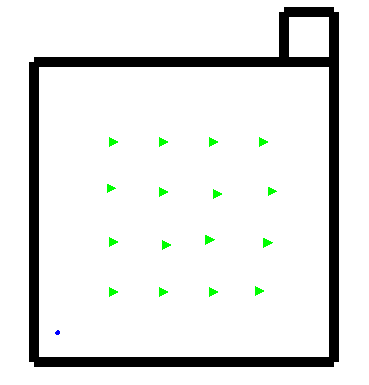
\includegraphics[scale=0.5]{figures/elderly_v2.png}
 \caption[頻尿の場合の可視化]{頻尿の場合の可視化 \label{elderly_v2}}
\end{center}
\end{figure}

\begin{figure}[htb]
\begin{center}
 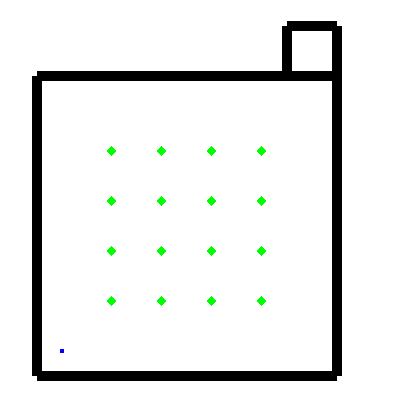
\includegraphics[scale=0.5]{figures/elderly_v3.png}
 \caption[認知症の場合の可視化]{認知症の場合の可視化 \label{elderly_v3}}
\end{center}
\end{figure}

ここでは,介護シミュレーションを可視化するために,これら3種類のエージェントを介護環境に配置する.それぞれが介護アラートを出す条件を,健常者の場合は100ml以上になった時点,頻尿の場合は75ml以上になった時点,認知症の場合は150ml以上で介護アラートを発する設定にし,アラートが発された時に被介護者とランダムにマッチングし,トイレへと向かうよう介護行動を設定した.この時,図\ref{care_alert_v1}のように,被介護者エージェントが介護アラートを出した時に、介護者エージェントが被介護者エージェントの元へ行き,トイレと連れて行く様子を可視化することができた.また,図\ref{alerts_v1}のように,複数の被介護者が同時に介護アラートを出した時は,介護者エージェントが介護すべき最適なエージェントの元へ行き,介護行動を行う様子も可視化することができた.そして図\ref{care_toilet_v1}のように,その介護が終わると同時に,残りの被介護者エージェントの元へと介護行動に向かわせることができた.したがって本シミュレーションは,介護環境を再現するのに必要最低限の機能を有したシミュレーションであると言える.なお,必要最低限の機能とは,被介護者がアラートを出した時点で,介護すべき最適な介護者とマッチングし,その介護者が適切に介護を行うことができることである.

\begin{figure}[htb]
\begin{center}
 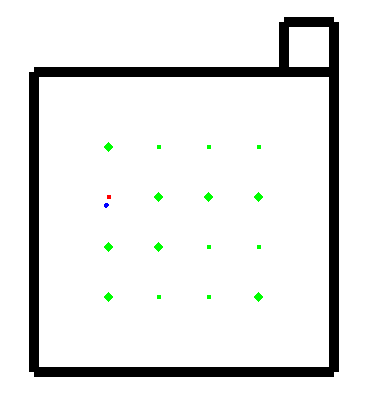
\includegraphics[scale=0.5]{figures/care_alert_v1.png}
 \caption[介護行動の可視化]{介護行動の可視化 \label{care_alert_v1}}
\end{center}
\end{figure}

\begin{figure}[htb]
\begin{center}
 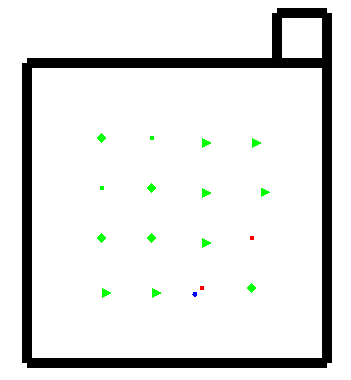
\includegraphics[scale=0.5]{figures/alerts_v1.png}
 \caption[複数介護アラートが出た場合の可視化]{複数介護アラートが出た場合の可視化 \label{alerts_v1}}
\end{center}
\end{figure}

\begin{figure}[htb]
\begin{center}
 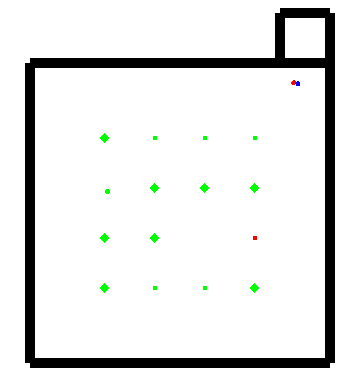
\includegraphics[scale=0.5]{figures/care_toilet_v1.png}
 \caption[介護行動の可視化]{介護行動の可視化 \label{care_toilet_v1}}
\end{center}
\end{figure}
